% ----------------------------------------------------------
% Resultados e Discussões
% ----------------------------------------------------------
\clearpage
\chapter{Resultados e Discussões}

Os testes foram realizados em pista oval com fita preta (largura 20\,mm) sobre superfície branca, em ambiente interno com iluminação artificial controlada. O protótipo operou de forma autônoma e contínua, sem intervenção humana após a inicialização, completando múltiplas voltas na pista. Todo o processamento ocorreu localmente no Raspberry Pi 4 a \textbf{20\,Hz}, com utilização média de CPU inferior a 15\%, demonstrando que a abordagem de \textit{Edge Computing} adotada é computacionalmente viável mesmo em hardware de baixo custo \cite{rpi4, rpi_network_throughput}. A comunicação serial permaneceu estável durante toda a sessão de testes, sem reinicializações nem erros de protocolo.

\section{Montagem e Sintonia do Controlador PID}
\label{sec:resultados_pid}

O chassi superior foi impresso em 3D (Autodesk Fusion 360), fixando o RPi4 na parte superior e o módulo BFD-1000 na extremidade frontal inferior. A sintonia dos ganhos seguiu o método empírico clássico: (1)~$K_p$ elevado até oscilação constante; (2)~$K_d$ introduzido para amortecer a oscilação em curvas agudas; (3)~$K_i$ mantido nulo, pois não houve acumulo de erro sistemático. A Tabela~\ref{tab:pid_tuning} consolida os parâmetros finais a 0{,}15 m/s de cruzeiro.

\begin{table}[H]
    \centering
    \caption{Parâmetros finais de sintonia do controlador PID.}
    \label{tab:pid_tuning}
    \small
    \begin{tabular}{|c|c|p{7cm}|}
        \hline
        \textbf{Ganho} & \textbf{Valor} & \textbf{Impacto no Comportamento} \\ \hline
        $K_p$ & $0{,}8$ & Correção enérgica em curvas agudas; evita saída da pista em chassi pesado. \\ \hline
        $K_i$ & $0{,}0$ & Nulo: sem erro de regime permanente nas retas avaliadas. \\ \hline
        $K_d$ & $0{,}2$ & Amortecimento crítico: elimina \textit{overshoot} e oscilação lateral (\textit{wobbling}). \\ \hline
    \end{tabular}
\end{table}

O ganho derivativo revelou-se o parâmetro mais crítico: a inércia rotacional do Roomba — não modelada pelo \textit{Turtlesim} — exigiu $K_d = 0{,}2$ para estabilizar a resposta. Com a sintonia final, os desvios laterais em retas foram zerados e as curvas fechadas foram percorridas com agilidade.

\section{Operação em Tempo Real}

Após a inicialização via \textit{launch file}, o nó \textit{line\_sensor\_node.py} publica as leituras binárias dos 5 sensores BFD-1000 no tópico \textit{/line\_sensor} a 20\,Hz. O nó \textit{pid\_controller\_node.py} subscreve esse tópico, calcula o erro por média ponderada ($\Delta t = 0{,}05$\,s), executa a Equação~\ref{eq:pid_discreto} e publica o comando resultante em \textit{/cmd\_vel}. O \textit{motor\_driver.py} converte a mensagem \textit{geometry\_msgs/Twist} para os bytes do protocolo Open Interface do Roomba, enviando-os via serial. Todo o grafo de comunicação é monitorável em tempo real pelo \textit{rqt\_graph} e pelo \textit{RViz2}, permitindo inspeção de latência e fluxo de dados sem parar o sistema. Nenhuma perda de pacote foi registrada nos testes, validando a estabilidade do \textit{middleware} DDS sob carga contínua a 20\,Hz. A Figura~\ref{fig:projeto_pronto} mostra o robô em operação na pista.

\begin{figure}[H]
    \centering
    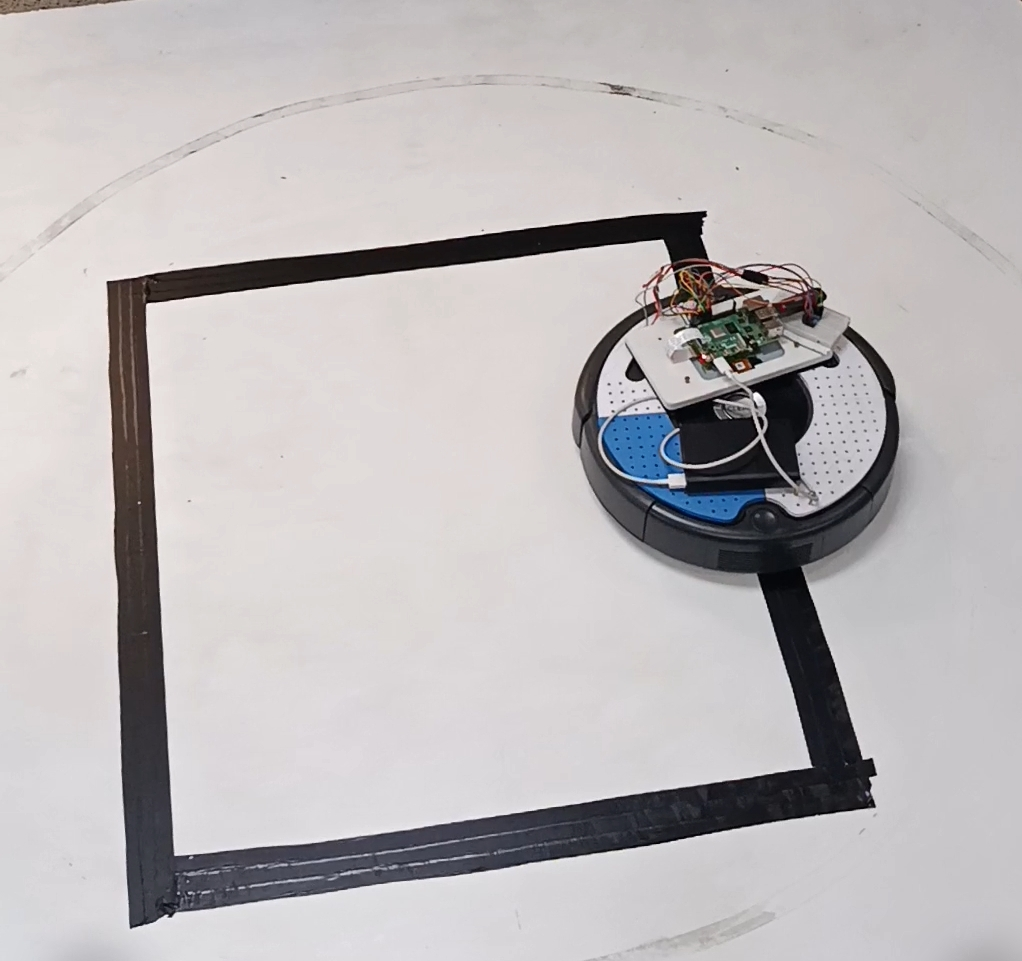
\includegraphics[width=0.42\textwidth]{imagens/roomba_funcionando_seguindo_linha}
    \caption{\label{fig:projeto_pronto}Robô em operação na pista de testes.}
    \legend{Fonte: Elaborado pelo autor.}
\end{figure}

A centralização do processamento no Raspberry Pi 4 eliminou camadas intermediárias de comunicação, reduzindo a latência entre detecção e atuação e validando a arquitetura \textit{Edge Computing} como viaável para controle robótico em tempo real. Nenhum pacote foi perdido nos testes, corroborando a estabilidade do \textit{middleware} DDS. Corroborando com \citeonline{Dantas_2022}, a plataforma consolida-se como recurso didático de alto valor para o ensino de PID, visão computacional e automação distribuída no LABIRAS/IFPI.
